\chapter{Propuesta}

Si bien el fin de este trabajo es postular un modelo que entregue los lineamientos generales para estimar la desviación en los costos de un proyecto de construcción minero basado en el nivel de madurez BIM 

\section{Métrica propuesta}

Si bien el fin de este trabajo es postular un modelo capaz de estimar los beneficios económicos asociados al uso del BIM en los proyectos de construcción minero-industriales en Codelco, el propósito general es que dicho modelo se pueda extender a cualquier tipo de proyecto de construcción, ya sea minero, industrial, de contrucción habitacional, etc.

%makes a littel sense though, like there's no real connection here

Además, dado el reducido número de proyectos que han adoptado la metología BIM en Codelco, es esencial que el método propuesto desestime el uso de un contrafactual para validarse, puesto que dicho método debe ser capaz de producir un modelo que pueda predecir los beneficios económicos en base al contexto particular de la industria de interés.

En este sentido, un método como el \citeA{barlish2012measure}, donde los indicadores propuestos permiten aventurar conclusiones en base a la comparación del nivel que estos alcanzaron en proyectos con BIM versus proyectos sin BIM, tiene la desventaja de necesitar de un contrafactual para validarse. Por otro lado, un método como el propuesto por \citeA{saldias2010estimacion}, que levanta conclusiones en base a la cantidad de SDIs y órdenes de cambio que pudieron haberse evitado con el uso de la metología BIM, tiene la desventaja de comparar proyectos sin BIM contra el ideal esperado con el uso de BIM, sin tomar en cuenta los puntos intermedios de proyectos que utilizan al menos algún nivel de esta metodología.

Por esta razón, este trabajo propone una metodología y una métrica que toman en cuenta las limitacions mencionadas, es decir, desestima el uso de un contrafactual y considera niveles intermedios del uso del BIM, y que, además, utiliza métodos estadísticos para validarlas.

La métrica propuesta sigue una línea metodológica similar a la mostrada por \shortciteA{lu2012generic}, donde el indicador es un parámetro derivado otros indicadores, que son los esfuerzos (medidos en HH) y la superficie por unidad de trabajo (m$^2$). 

Así, en vez de construir un modelo en base a indicadores que pueden extraerse de manera directa de los reportes de los proyectos, el modelo propuesto utiliza una métrica que toma en cuenta el nivel de madurez BIM alcanzado (de acuerdo a una escala previamente determinada), el nivel óptimo de madurez y la desviación de los costos de los proyectos.

Asimismo, y dado que se espera que los costos de un proyecto crezcan en relación inversa al nivel de madurez BIM alcanzado por este, es necesario que el indicador se compare con respecto a su nivel de madurez óptimo. Formalmente, esto queda:

\begin{equation}
    \text{Indicador Madurez} = \frac{\text{Madurez BIM óptima}}{\text{Nivel madurez BIM}}
\end{equation}

\section{Selección y generación de datos}

\subsection{Criterio de selección}

Para poder generar un modelo que permita validar el uso del indicador propuesto, la información sobre la cuál se compara dicho parámetro es la desviación de los costos en un proyecto determinado, y, en particular, la desviación en costos que tenga relación directa con la falta de integración de la metodología BIM. En otras palabras, la información relevante es la relativa a todos aquellos factores que devinieron en un aumento de costos y que pudieron evitarse de haberse utilizado e integrado el BIM de manera óptima.

De esta manera, la selección de los datos utilizados para relacionar estas variables y generar un modelo capaz de predecir la desviación en costos basasado en la métrica propuesta tuvo dos fuentes principales de las cuales se extrajo la información: el reporte final de los proyectos con los cambios y tendencias, y el detalle de los contratos de cada proyecto.

Sin embargo, dado el nivel de detalle de la información contenida, se escogió el reporte con el detalle de los contratos como fuente de extracción de datos. Además, dicho reporte separa el detalle del costo base y el costo final. Esta clasficiación permite generar una estructuta de filtrado de datos que sigue la siguiente selección jerarquizada:

\begin{enumerate}
    \item \textbf{Contratos que crecieron:} primero, se seleccionan todos los contratos que experimentan un crecimiento en sus costos respecto del presupueto base.
    
    \item \textbf{Sólo crecimientos:} luego, se considera sólo la información referida a los crecimientos de los costos de cada contrato, desestimándose la información detallada sobre el costo base de estos.
    
    \item \textbf{Itemización BIM:} finalmente, se separa la información por ítems relacionados al uso (o falta de uso) de BIM. La itemización BIM se compone de los siguientes ítems: extensión de plazo, obras adicionales, materiales e ingeniería.
\end{enumerate}

La selección de información asociada a cada uno de los ítems de la itemización BIM puede variar según el proyecto. Sin embargo, para el caso de los proyectos analizados en este estudio, las palabras clave para dicha selección eran coincidentes entre proyectos. Esto dado que quienes crean el reporte son parte de la misma Dirección (Dirección de Contratos) y de la misma compañía (Codelco). 

Se tiene, entonces, que para el filtrado por ítem, las palabras clave fueron:

\begin{table}[H]
    \centering
    \caption{Palabras clave para la selección de cada ítem asociado al BIM.}
    \label{tab.keyw}
    \begin{tabular}{ll}
        \toprule
        \textbf{Ítems} & \textbf{Palabras clave} \\
        \midrule
        Extensión de plazo & Extensión plazo, plazo\\
        Obras adicionales & Montaje, obras adicionales, rellenos, reemplazos, reparaciones, etc.\\
        Materiales & Hormigón, piping, cañerías, cables, válvulas, etc. \\
        Ingeniería & Ingeniería, ingeniería de terreno, etc. \\
        \bottomrule
    \end{tabular}
\end{table}

Una vez seleccionada toda la información asociada a cada ítem, se calcula el porcentaje que representa cada uno de ellos respecto del presupuesto base y se genera un nuevo set de datos que representa la desviación en costos asociada al uso del BIM por cada uno de los proyectos.

Luego, las desviaciones en costos para los proyectos estudiados en este trabajo se distribuyen de acuerdo a lo mostrado en la siguiente Tabla:

\begin{table}[H]
    \centering
    \label{tab.datos_desv_proy}
    \caption{Desviaciones en costo de los proyectos estudiados.}
    \begin{tabular}{lccc}
        \toprule 
        Ítem & MH & Molyb & Planta de Ácido \\
        \midrule
        Extensión plazo & 2,0 \% & 5,4 \% & - \\
        Obras adicionales & 19,7 \% & 2,4 \% & 5,6 \%\\
        Materiales & 3,2 \% & 8,1 \% & 5,9\% \\       
        Ingeniería & 0,08 \% & 0,12 \% & 0,3 \% \\
        \textbf{Total} & 25,0 \% & 16,2 \% & 11,8 \% \\
        \bottomrule
    \end{tabular}
\end{table}

\subsection{Herramienta de selección y generación de base de datos}

El reporte con el detalle de los contratos es una planilla Excel con miles de datos, por lo que el filtrado a través de este mismo software no es conveniente. Por esta razón, se creó un código en Python para la selección de los datos requeridos a través de una pseudo minería de datos \footnote{Disponible en \url{www.github.com/psotou/contract-data-selection.git} }. Cabe mencionar que si bien el código se creó para trabajar con cualquier reporte de detalle de contratos emitidos por la Vicepresidencia de Proyectos de Codelco, basta con ajustar algunos parámetros para que dicho código pueda usarse con un reporte de similares características de cualquier otra compañía.

Así, una vez generado el conjunto de datos asociado a las desviaciones en costos, se procede a estimar los resultados arrojados por la métrica propuesta. Para ello, se consultó la opinión experta de Marcelo Vásquez, quien fue el coordinador BIM de todos los proyectos estudiados. 

Ha de mencionarse que la madurez BIM se puede medir usando la métrica o metodología que más convenga, sin embargo, en este estudio se decidió por el uso de la matriz de madurez propuesta por Succar \cite{succar2010building}. Dicha matriz entrega un rating que va del 1 al 4, siendo 4 el óptimo de madurez. Bajo este contexto, la evaluación de Marcelo Vásquez para los proyectos fue la siguiente:

\begin{table}[H]
    \centering
    \label{tab.datos_mad_bim}
    \caption{Nivel de madurez BIM de cada proyecto.}
    \begin{tabular}{lc}
        \toprule 
        \textbf{Proyecto} & \textbf{Nivel de madurez BIM} \\
        \midrule
        Ministro Hales & 1,7 \\
        Moly corporativo & 2,2 \\
        Planta de ácido &  1,8 \\
        \bottomrule
    \end{tabular}
\end{table}

Aplicando la transformación propuesta como indicador (a la que en adelante se referirá como madurez por simplicidad), el conjunto de datos sobre los que se levanta la propuesta de este estudio queda como sigue:

\begin{table}[H]
    \centering
    \label{tab.datos_mad_bim_desv}
    \caption{Base de datos desviación de costos (crecimientos) e indicador madurez.}
    \begin{tabular}{lcc}
        \toprule 
        \textbf{Proyecto} & \textbf{Desviación} & \textbf{Madurez} \\
        \midrule
        Ministro Hales & 25,0 \% & 2,35 \\
        Moly corporativo & 16,2 \% & 1,82 \\
        Planta de ácido & 11,8 \% & 2,22 \\
        \bottomrule
    \end{tabular}
\end{table}


En base a esta información se construye el modelo que permite predecir la desviación en costos de un proyecto de acuerdo a su nivel de madurez BIM.

%-----------------------------MODELO TEÓRICO----------------------
\section{Teoría del modelo propuesto}

En términos generales, la relación entre desviación en costos de un proyecto $i$ y los factores que la motivan se puede expresar de la siguiente manera:

\begin{equation}
    \label{eq.desv-gen}
    y_i = \theta_0 +\sum\limits_{i=1}^n \theta_i x_i
\end{equation}

O bien, de manera vectorial:

\begin{equation}
    \label{eq.desv-vec}
    y_i = \bm{x}^T_i\bm{\theta}
\end{equation}

Donde tanto $y_i$ como $\bm{x}_i$ son variables observadas. Se asumirá que $\varepsilon_i$ (término de error o de perturbación no observado) es absorbido por la constante $\theta_0$. Aquí, $\bm{x}^T$ es un vector fila cuyos elementos son los indicadores de madurez propuestos $(1,~x_1,~x_2,\ldots,~x_n)$, y $\bm{\theta}$ es un vector columna con $(\theta_0,~\theta_1,~\theta_2,\ldots,~\theta_n)^T$  paramámetros desconocidos que son los que se desea estimar para generar un modelo capaz de explicar la influencia de factores tales como el uso de alguna nueva metodología (que es el caso de este estudio), clima, paralizaciones, etc, en la desviación de los costos de un proyecto y, adicionalmente, predecir este resultado.

En este trabajo, $y_i$ representa las desviaciones en costos para el proyecto $i$, y $\bm{x}_i$ es el indicador de madurez propuesto.


Además, la ecuación \eqref{eq.desv-vec} se puede escribir usando notación matricial:

\begin{equation}
    \label{eq.matrix}
    \bm{y} = X\bm{\theta} + \varepsilon
\end{equation}

Donde $\bm{y}$ y $\varepsilon$ son vectores de dimensiones $(N\times1)$, $X$ es una matriz de dimensión $(N\times K)$ y $\bm{\theta}$ un vector de dimensión $(K\times1)$.

Antes de comenzar con la estimación de los parámetros de interés $\bm{\theta}$, se deben levantar algunos supuestos para darle significado al modelo de manera que este no carezca de sentido estadístico. En primer lugar, se asume que las variables explicativas $\bm{x}_i$ son exógenas, lo que implica que $\bm{E}[y_i|\bm{x}_i]=0$. Bajo este supuesto, se sostiene que :

\begin{equation}
    \label{eq.e-xb}
    \bm{E}[y_i|\bm{x}_i] = \bm{x}_i^T\bm{\theta}
\end{equation}

De manera que la curva $\bm{x}_i^T\bm{\theta}$ describe la esperanza condicional de $y_i$ dados los valores de $\bm{x}_i$, y los coeficientes de $\bm{\theta}$ miden cuánto cambia el valor esperado de $y_i$ si cambia un valor $x_{ik}$ (siendo éste el $k$-ésimo elemento del vector $\bm{x}_i$) manteniendo todos los otros elementos de $\bm{x}_i$ constantes (condición ceteris paribus) \cite{verbeek}.

Los parámetros de $\bm{\theta}$ se estimarán on el estimador de Mínimos Cuadrados Ordinarios (MCO). Utilizando la notación de la ecuación \eqref{eq.matrix}, el estimador está dado por:

\begin{equation}
    \label{eq.mco}
    \bm{\hat\theta} = \left( X^TX\right)^{-1}X^T\bm{y}
\end{equation}

Luego, la predicción de valores de desviación vendrá dada por:

\begin{equation}
    \label{eq.predicc}
    \hat{\bm{y}} = X\hat{\bm{\theta}}
\end{equation}

Donde $\hat{\bm{y}}$ son las predicciones de las desviaciones dada la estimación de los parámetros de $\bm{\theta}$.  

La muestra sobre la cual se funda este estudio consiste de un conjunto muy reducido de datos, por lo que se utilizará MCO para muestra pequeña. Las propiedades del estimador MCO para muestra pequeña son:

\begin{align}
    & \label{eq.s1} \bm{E}[\varepsilon_i] = 0\\
    & \label{eq.s2} \varepsilon_i\quad\text{independiente de}\quad \bm{x}_i\\
    & \label{eq.s3} \bm{V}[\varepsilon_i]=\sigma^2 \\
    & \label{eq.s4} \text{cov}[\varepsilon_i,~\varepsilon_j] = 0,\quad i\neq j
\end{align}

El supuesto \eqref{eq.s1} indica que el valor esperado del término de error es cero, esto significa que, en promedio, la curva de regresión debería estar correcta. El supuesto \eqref{eq.s3} indica que todos los términos de error poseen la misma varianza, esto se conoce como homoceasticidad, mientras que supuesto \eqref{eq.s4} impone cero correlación entre los términos de error, excluyende así cualquier forma de autocorrelación. Usando la notación matricial, estos tres supuesto se pueden reescribir de la siguiente forma:

\begin{equation}
    \bm{E}[\varepsilon]=0\quad\text{y}\quad\bm{V}[\varepsilon]=\sigma^2I_N
\end{equation}

Con $I_N$ matriz identidad de dimensiones $(N\times N)$. Esto muestra que la matriz de covarianza del vector de los términos de error $\varepsilon$ es una matriz diagonal con $\sigma^2$ en la diagonal.

El supuesto \eqref{eq.s2} indica que $X$ e $\varepsilon$ son independientes. Este es un supuesto fuerte que implica:

\begin{equation}
    \bm{E}[\varepsilon|X]=\bm{E}[\varepsilon]=0
\end{equation}
\begin{equation}
    \bm{V}[\varepsilon|X]=\bm{V}[\varepsilon]=\sigma^2I_N
\end{equation}

Es decir, la matriz de regresores $X$ no provee ninguna información sobre los valores esperados de los términos de error o sus (co)varianzas. 

Una propiedad muy relevante del estimador de mínimos cuadrados es que se trata de un \textbf{estimador insesgado}. Esto quiere decir que, en promedio, se espera que los valores del estimador $\bm{\hat\theta}$ sean iguales a los valores verdaderos de $\bm{\theta}$ \cite{verbeek}. Formalmente, esto es:

\begin{equation}
    \bm{E}[\hat{\bm{\theta}}] = \bm{\theta}
\end{equation}

Hasta ahora se ha descrito la interpretación del modelo para un valor esperado de $y_i$ dados los valores observado de las variables explicativas $\bm{x}_i$.

Además de ese análisis, es importante conocer el \textbf{efecto marginal} de dichas variables sobre el valor esperado de $y_i$. En otras palabras, en cuántas unidades se espera que cambie $y_i$ si $x_{ik}$ cambia en una unidad siempre que el resto de las variables en $\bm{x}_i$ se mantenga constante (condición ceteris paribus) \cite{hansen2018}. Esta medida viene dada por:

\begin{equation}
    \label{eq.efec_marginal}
    \frac{\partial \bm{E}[y_i|\bm{x}_i]}{\partial x_{ik}} =\theta_k
\end{equation}

%--------------------------MODELO EMPÍRICO---------------
\section{Modelo propuesto}

La coordinación digital de un proyecto de construcción a través del uso de la metodología BIM supone reducir los costos asociados a errores, interferencias, omisiones, etc, por lo que a medida que el grado de integración de la metodología en el proyecto crece, los costos asociados a los problemas mencionados disminuyen.

Dado este escenario, es de esperarse que el uso del BIM impacte de manera postiva en el ahorro en costos de construcción de un proyecto. Se desprende, entonces, que un proyecto que alcanza un buen nivel de madurez BIM debería tener un sobre costo menor al esperado en un proyecto realizado sin BIM.

Por lo anterior, la hipótesis sobre la que se basa esta propuesta es que la desviación de los costos de un proyecto es inversamente proporcional a su grado de madurez BIM. Para ello, se define la variable explicativa $x_{ik}$ de la siguiente manera:

\begin{equation}
    x_{ik} = \frac{m}{m_i}
\end{equation}

Donde $m$ es el óptimo de madurez BIM, y $m_i$ es el nivel de madurez BIM alcanzado por el proyecto $i$. 

Con esto, la ecuación \eqref{eq.desv-gen} queda:

\begin{equation}
    y_i = \theta_0 + \sum\limits_{i=1}^n \theta_i \left(\frac{m}{m_i} \right)
\end{equation}

Además, la desviación en los costos de un proyecto está sujeta las siguientes condiciones de borde de acuerdo a la NBS \cite{nbs}:

\begin{equation}
    y_i = 
    \begin{cases}
        0,33 & \text{si}~~ m_i = m_{\text{máx}} \\
        0,001 & \text{si}~~ m_i = m_{\text{mín}}
    \end{cases}
\end{equation}

La muestra de la que se disponía y sobre la que se trabajó, consistía de tres proyectos minero-industriales, dos de estos proyectos de construcción greenfield mientras que el otro, un proyecto de overhauling. Por esta razón, se realiza un análisis para la submuestra de elementos homogéneos y otro para el total de la muestra.

%--------------------SUBMUESTRA HOMOGÉNEA-------------------------------
\subsection{Submuestra homogénea}

Este análisis considera la submuestra de los proyectos greenfield, que además compartían la construcción del mismo número de plantas de procesamiente, aunque para minerales distintos. Los datos de desviación de costos, madurez BIM y condiciones de borde son los siguientes:

\begin{minipage}{.45\linewidth}
    \begin{equation*}
    Y = 
        \begin{bmatrix}
            0,330 \\
            0,249 \\
            0,161 \\
            0,001 
        \end{bmatrix}
    \end{equation*}
\end{minipage}
\begin{minipage}{.45\linewidth}
    \begin{equation*}
    X = 
        \begin{bmatrix}
            1 & & 4,000 \\
            1 & & 2,353 \\
            1 & & 1,818 \\
            1 & & 1,000
        \end{bmatrix}
    \end{equation*}
\end{minipage}

Esto genera el estimador:

\begin{equation}
    \hat{\bm{\theta}} = 
        \begin{bmatrix}
            -0,0532 \\
            ~~~0,1040
        \end{bmatrix}
\end{equation}

Este resultado genera la siguiente relación:

\begin{equation}
    \label{eq.modelo-prop-submuestra}
    y_i = -0,0532 + 0,104\cdot \left( \frac{4}{m_i} \right)
\end{equation}

Cuyo efecto marginal sobre la desviación esperada de los costos es $0,104$. Es decir, por cada una unidad de madurez BIM se espera una reducción en la desviación esperada de aproximadamente un $10,4\%$.

La escala con la que se mide madurez BIM para este estudio toma valores que van desde el 1 al 4, con un error asociado de $\pm 0,05$. Tomando en cuenta este rating, se genera un gráfico con la predicción de la desviaciones en costos en base al nivel de madurez.

\begin{figure}[H]
    \centering
    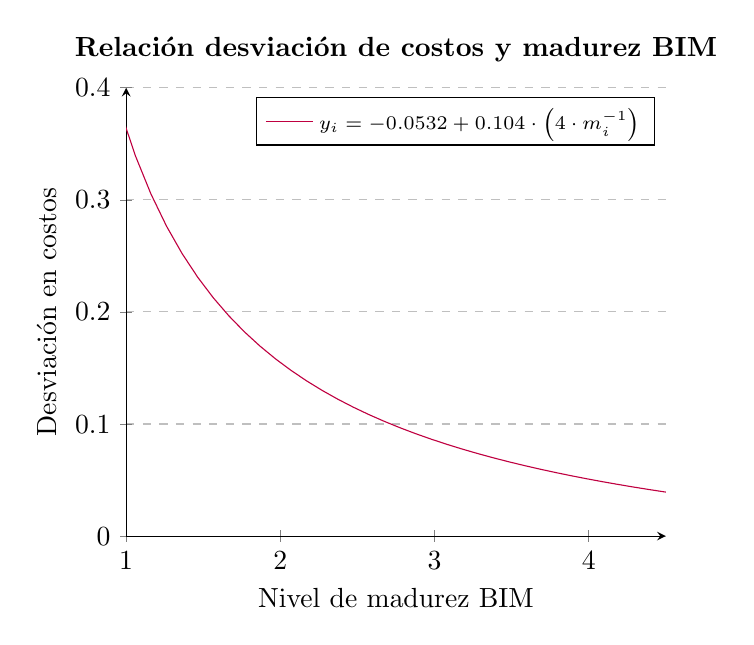
\begin{tikzpicture}
        \begin{axis}[
            axis lines = left,
            title = {\textbf{Relación desviación de costos y madurez BIM}},
            ymin = 0, ymax = 0.4,
            xmin = 1, xmax = 4.5,
            xtick = {1, 2, 3, 4},
            ymajorgrids = true,
            grid style = dashed,
            ylabel = Desviación en costos,
            xlabel = Nivel de madurez BIM,
            legend style = {font=\scriptsize},
         ]
        \addplot [
            samples = 100,
            color = purple,
         ]
         {-0.0532+0.104*4/x};
         \addlegendentry{$y_i = -0.0532 + 0.104 \cdot \left( 4\cdot m_i^{-1} \right)$}
        \end{axis}
    \end{tikzpicture}
    \caption{Predicción de la desviación en costos en base a la submuestra homogénea.}
\end{figure}

Las estadísticas asociadas al coeficiente que acompaña la relación de madurez BIM se muestran en la siguiente Tabla:

\begin{table}[H]
    \centering
    \label{tab.est}
    \caption{Estadísticas asociadas al coeficiente de madurez BIM $\theta_1$.}
    \begin{tabular}{lccc}
        \toprule
        Coeficiente & error estándar & $p$-value & $R^2$\\
        \midrule
        0,104 & 0,028 & 0,065 & 0,87\\  
        \bottomrule        
    \end{tabular}
\end{table}

%---------------------MUESTRA TOTAL--------------------------
\subsection{Muestra Total}

Ahora, ingresando los datos de desviación y madurez de toda la muestra, se generan las siguientes matrices:

\begin{minipage}{.45\linewidth}
    \begin{equation*}
    Y = 
        \begin{bmatrix}
            0,330 \\
            0,249 \\
            0,161 \\
            0,118 \\
            0,001 
        \end{bmatrix}
    \end{equation*}
\end{minipage}
\begin{minipage}{.45\linewidth}
    \begin{equation*}
    X = 
        \begin{bmatrix}
            1 & & 4,000 \\
            1 & & 2,353 \\
            1 & & 1,818 \\
            1 & & 2,222 \\
            1 & & 1,000
        \end{bmatrix}
    \end{equation*}
\end{minipage}

Lo que produce el siguiente estimador:

\begin{equation}
    \hat{\bm{\theta}} = 
        \begin{bmatrix}
            -0,0667 \\
            ~~~0,1047
        \end{bmatrix}
\end{equation}

Con lo que la relación entre desviación y madurez se modela como sigue:

\begin{equation}
    \label{eq.modelo-prop-todos}
    y_i = -0,0667 + 0,1047\cdot \left( \frac{4}{m_i} \right)
\end{equation}

Cuyo efecto marginal sobre la desviación esperada de los costos es $0,1047$. Es decir, por cada una unidad de madurez BIM se espera una reducción en la desviación esperada de aproximadamente un $10,5\%$.

El gráfico asociado a la ecuación \eqref{eq.modelo-prop-todos} es:

\begin{figure}[H]
    \centering
    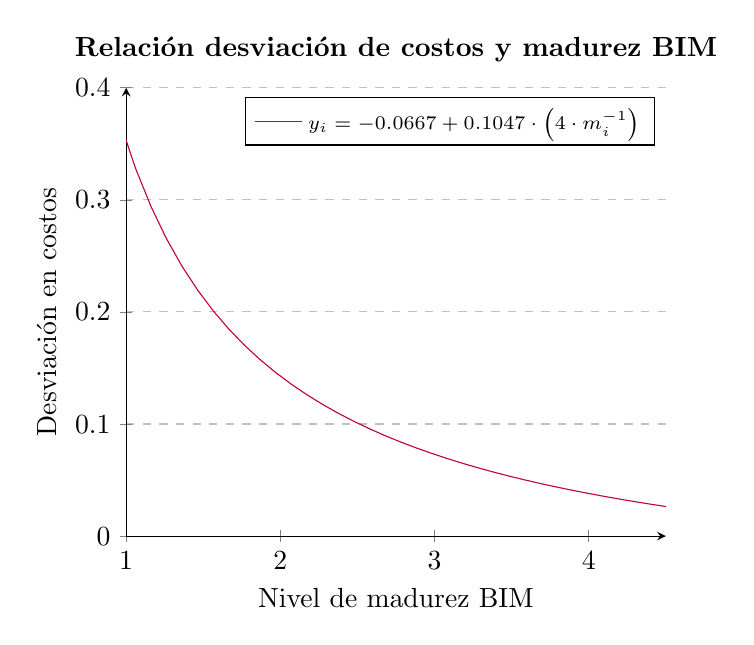
\begin{tikzpicture}
        \begin{axis}[
            axis lines = left,
            title = {\textbf{Relación desviación de costos y madurez BIM}},
            ymin = 0, ymax = 0.4,
            xmin = 1, xmax = 4.5,
            xtick = {1, 2, 3, 4},
            ymajorgrids = true,
            grid style = dashed,
            ylabel = Desviación en costos,
            xlabel = Nivel de madurez BIM,
            legend style = {font=\scriptsize},
         ]
        \addplot [
            samples = 100,
            color = purple,
         ]
         {-0.0667+0.1047*4/x};
         \addlegendentry{$y_i = -0.0667 + 0.1047\cdot \left( 4 \cdot m_i^{-1} \right)$}
        \end{axis}
    \end{tikzpicture}
    \caption{Predicción de la desviación en costos en base a la muestra total.}
\end{figure}

Y las estadísticas asociadas al coeficiente que acompaña la relación de madurez BIM se muestran en la siguiente Tabla:

\begin{table}[H]
    \centering
    \label{tab.est}
    \caption{Estadísticas asociadas al coeficiente de madurez BIM $\theta_1$.}
    \begin{tabular}{lccc}
        \toprule
        Coeficiente & error estándar & $p$-value & $R^2$\\
        \midrule
        0,1047 & 0,027 & 0,03 & 0,83\\  
        \bottomrule        
    \end{tabular}
\end{table}

Si se comparan las curvas generadas a partir tanto de la submuestra como de la muestra total, se puede apreciar un desplazamiento en favor de la curva generada por el modelo derivado de la muestra total (pues se acerca más a las condiciones de borde que indica la teoría).

\begin{figure}[H]
    \centering
    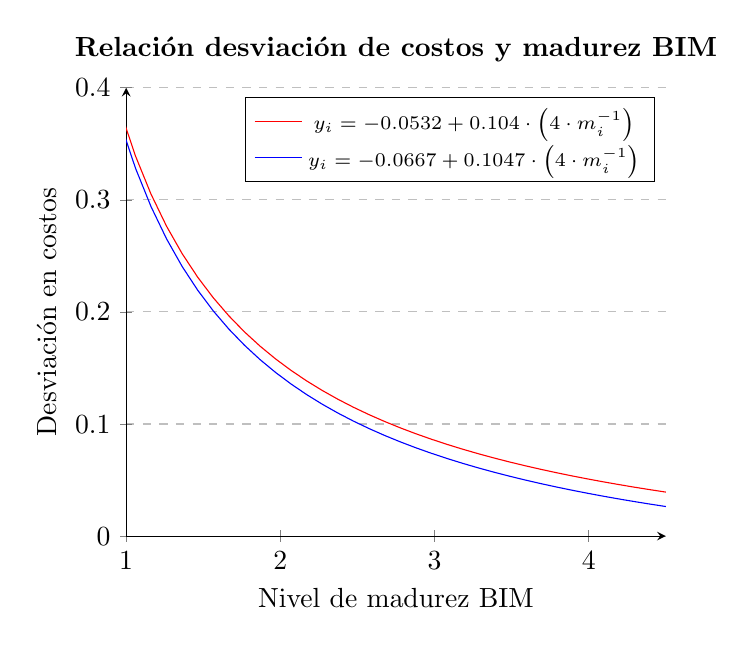
\begin{tikzpicture}
        \begin{axis}[
            axis lines = left,
            title = {\textbf{Relación desviación de costos y madurez BIM}},
            ymin = 0, ymax = 0.4,
            xmin = 1, xmax = 4.5,
            xtick = {1, 2, 3, 4},
            ymajorgrids = true,
            grid style = dashed,
            ylabel = Desviación en costos,
            xlabel = Nivel de madurez BIM,
            legend style = {font=\scriptsize},
        ]
        \addplot [
            samples = 100,
            color = red,
        ]
        {-0.0532+0.104*4/x};
        \addlegendentry{$y_i = -0.0532 + 0.104 \cdot \left( 4\cdot m_i^{-1} \right)$}
        %second plot
        \addplot [
            samples = 100,
            color = blue,
        ]
        {-0.0667+0.1047*4/x};
        \addlegendentry{$y_i = -0.0667 + 0.1047\cdot \left( 4 \cdot m_i^{-1} \right)$}
        \end{axis}
    \end{tikzpicture}
    \caption{Diferencia de predicciones entre el modelo propuesto en base a la submuestra homogénea (línea roja) y a la muestra total (línea azul).}
\end{figure}


%------------RESULTS ANALYSIS----------------
\subsection{Análisis de Resultados}

Como se mencionó más arriba, la propuesta de este estudio se basa en mostrar la relación inversa entre desviación de costos y madurez BIM y, junto a esto, validar la métrica propuesta a través de métodos estadísticos. Así, la hipótesis que se sostiene es que, efectivamente, existe una relación entre estas variables y dicha relación es inversamente proporcional. Formalmente:

\begin{table}[H]
    \begin{tabular}{l p{0.9\linewidth}}
        $H_0$: & La madurez BIM no tiene un efecto inversamente proporcional a la desviación en los costos de construcción de un proyecto. \\

        $H_1$: & La madurez BIM sí tiene un efecto inversamente proporcional a la desviación en los costos de construcción de un proyecto.
    \end{tabular}
\end{table}

Donde $H_0$ es la hipótesis nula y $H_1$ la hipótesis alternativa. 

Para validar el modelo propuesto en términos estadísticos se debe contar con evidencia para rechazar $H_0$. La manera de corroborar dicha información es tomando el cuenta el valor que muestra el $p$-value. Puesto de otra manera, si $p<0,05$ existe evidencia para rechazar $H_0$; de lo contrario, si $p>0,05$, la evidencia en contra de $H_0$ es débil y no se puede rechazar. 

En este caso, y a pesar de lo limitada de la muestra, se tiene que para la submuestra de elementos homogéneos $p>0,05$, por lo que evidencia para rechazar $H_0$ es débil.

Por otro lado, al considerar la muestra total se tiene que $p<0,05$, de manera que se puede rechazar $H_0$ en favor de $H_1$, indicando así que existe evidencia estadística para validar la hipótesis de la relación inversa entre madurez BIM y desviación de costos.

Así, tomando en cuenta el resultado arrojado por la muestra total, el modelo representado en la ecuación \eqref{eq.modelo-prop-todos} sería el adecuado para predecir las desviación en costos de cualquier proyecto considerando únicamente su nivel de madurez BIM respecto de un óptimo. 

Sin embargo, y a pesar de que si bien el resultado de la muestra total se condice con lo esperado en teoría, ha de tenerse en cuenta que se utilizó una muestra bastante acotada, por lo que se debe tener el cuidado pertinente si se quiere generalizar sobre este resultado. No obstante, el modelo propuesto se comporta de manera bastante apropiada y viene a validar, en términos cuantitavos, aquella \emph{sensación} de ahorro que genera la utilización de la metodología BIM.